Welch's method is a modified type of periodogram. Instead of transforming the whole input sequence into the frequency domain, the sequence is split into multiple overlapping\footnote{without overlapping, this method is called ``Bartlett's Method''} intervals (windowed). Then, all the individual power spectra of these intervals are calculated and averaged to produce the final periodogram. The overlapping of the segments can help to restore some of the power content on the edges of the segments that was lost due to windowing. Figure \ref{fig:welch_ill} shows an illustration of this method.\\

\begin{figure}[h]
\centering
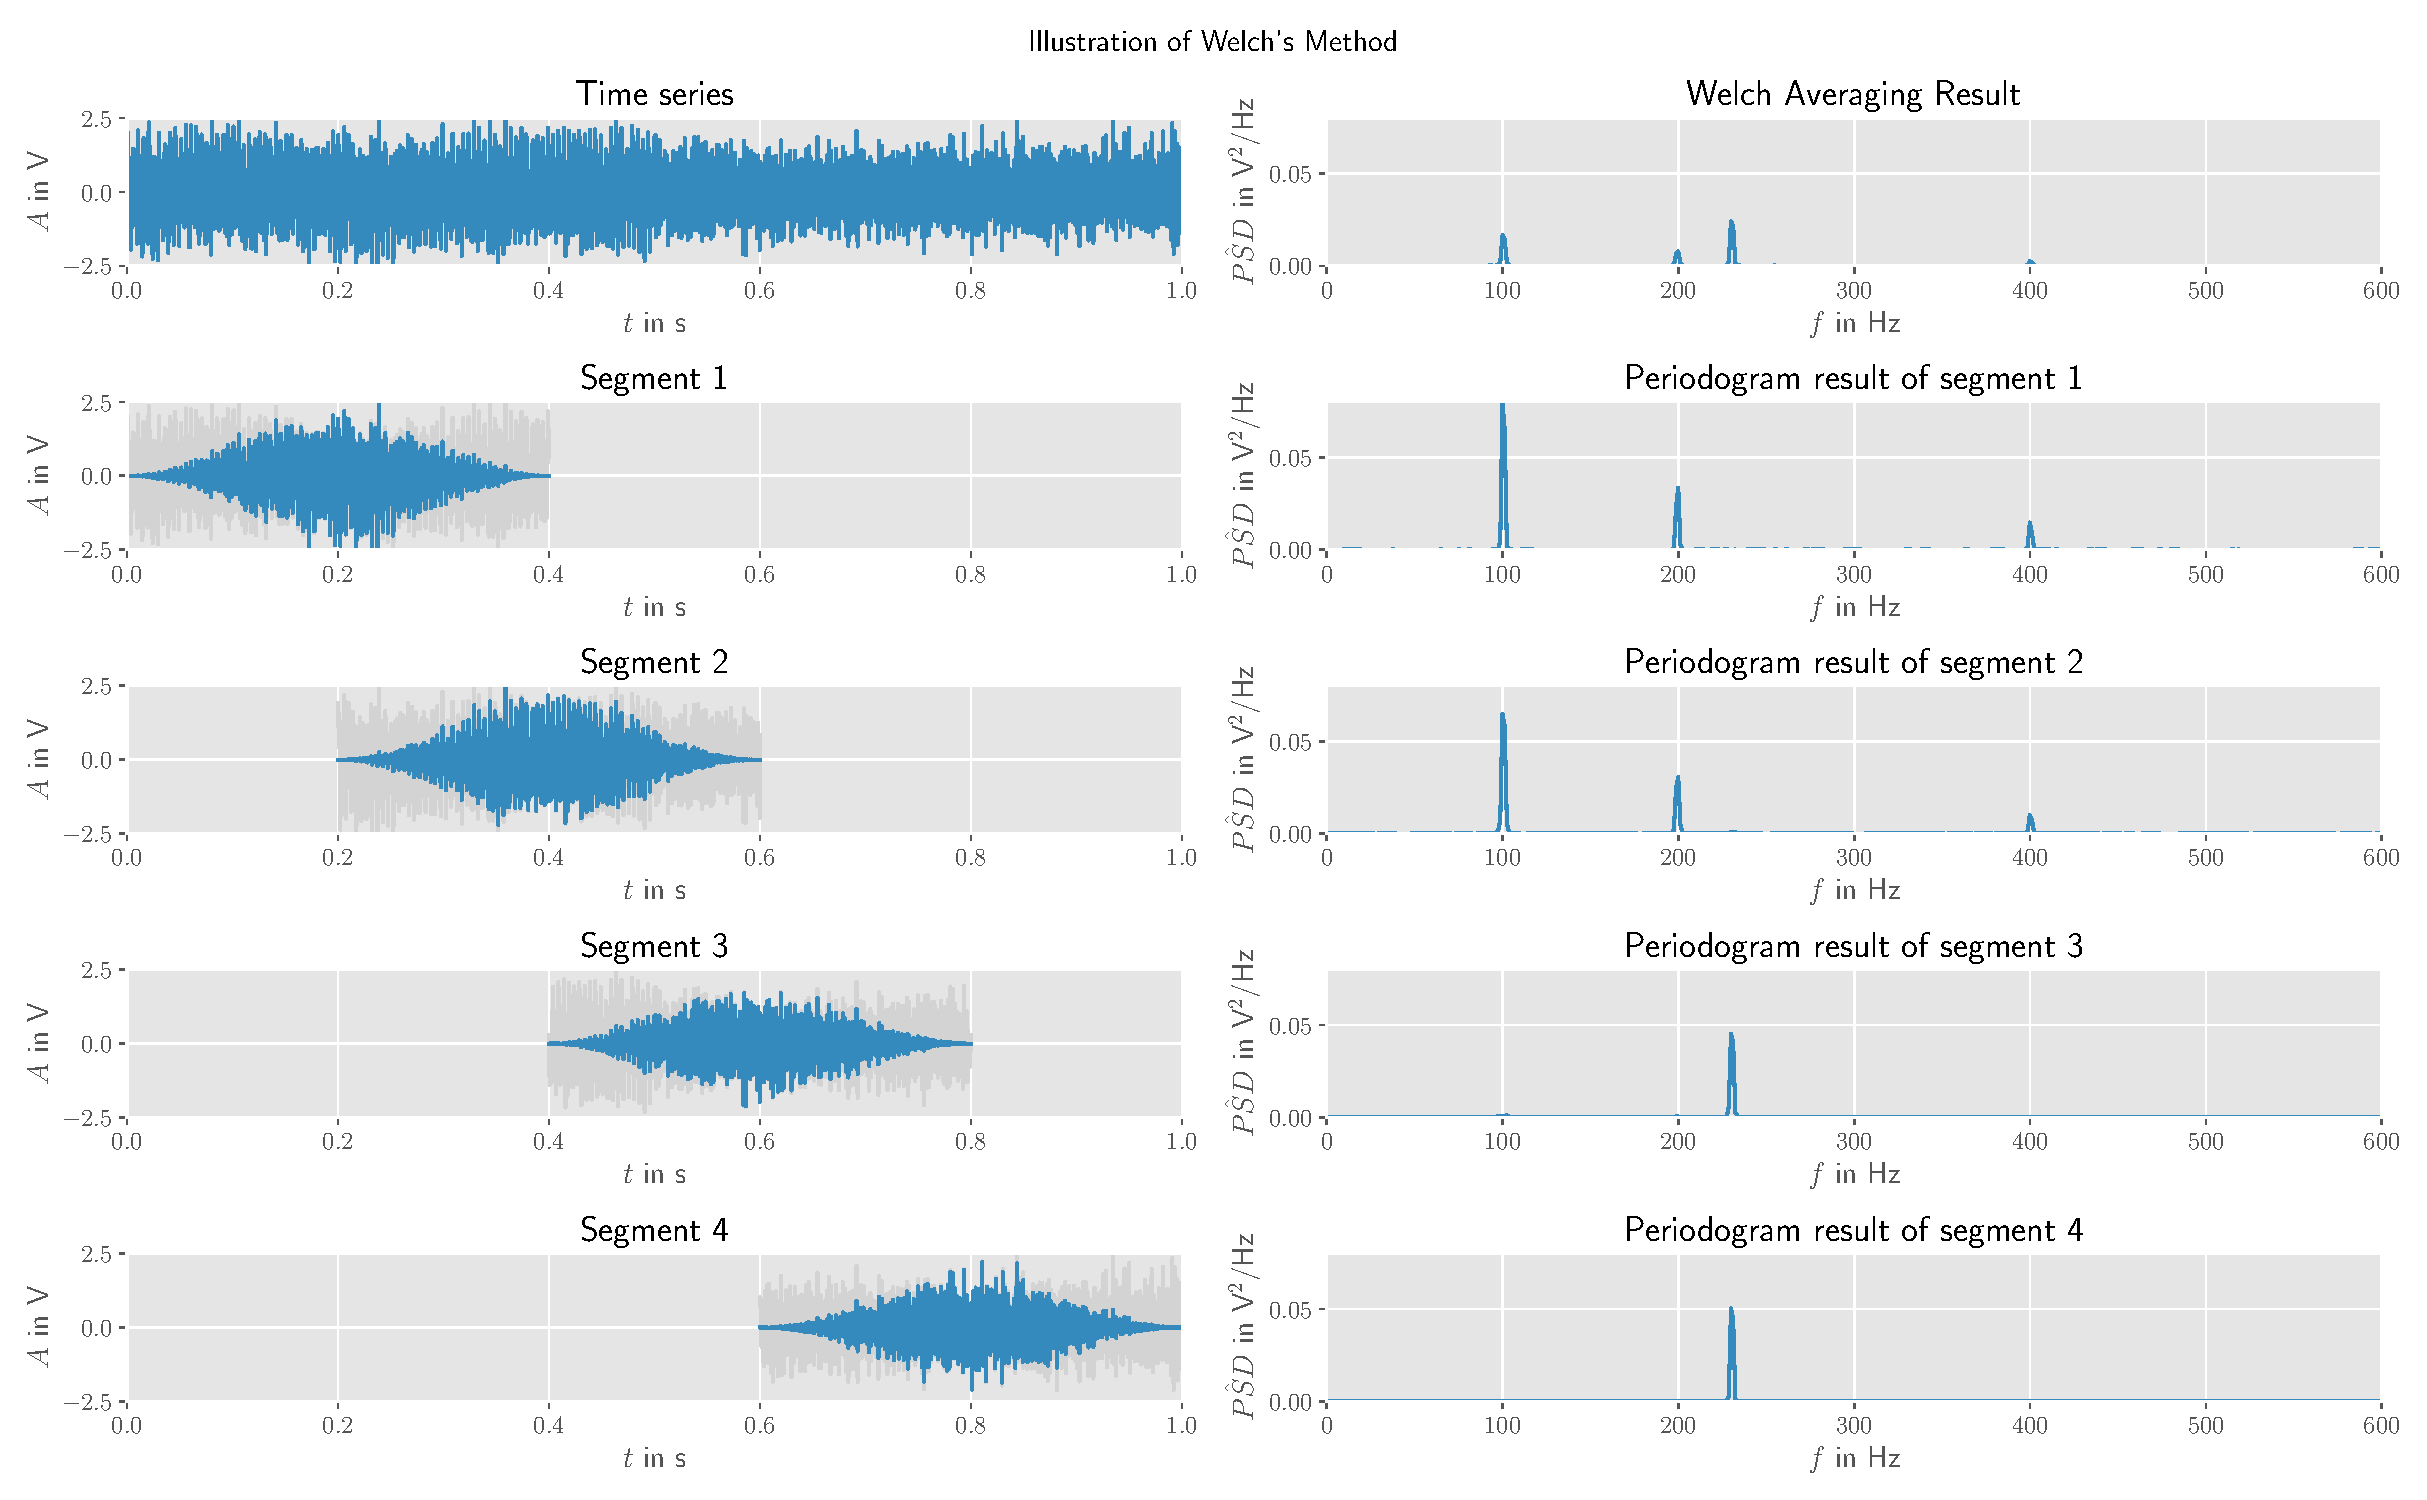
\includegraphics[width=\textwidth]{graphics/welch_illustration.pdf}
\caption{Illustration of Welch's method. The time series is split into multiple windowed segments which are then individually transformed into periodograms that are averaged to obtain the overall periodogram. In this case, the 4 segments were windowed with a Hann window. The total size is $N= 6000$.}\label{fig:welch_ill}
\end{figure}

Due to the averaging approach of Welch's method, the resulting periodogram might be less sensitive to noise in the time series. E.g. think about a short-duration noise spike in the data: In the full FFT, it might introduce large high frequency content but in the Welch periodogram it will only be evaluated in a fraction of the segments and therefore might not be visible after averaging.\\

However, since the splitting of the sequence into segments reduces the time window of each individual FFT, the frequency resolution will be smaller than the FFT of the whole sequence ($\frac{1}{T_{w}}$).
This can become a problem when trying to distinguish harmonics of the signal that are relatively closely spaced in frequency.\\

Adjustable parameters of this method include the segment size, the overlapping size, and the window applied.

Figure \ref{fig:welch_exp} shows the periodograms of both test signals and compares them to the standard periodogram. The noise level has been reduced by the Welch periodogram. However, the frequencies of signal $B$ are not distinguishable anymore due to the reduced frequency resolution. The code for this can be found in appendix \ref{app:welch}. Figure \ref{fig:welch_comp} further shows that the application of the Welch window requires a tradeoff of its parameters.

\begin{figure}[h]
\centering
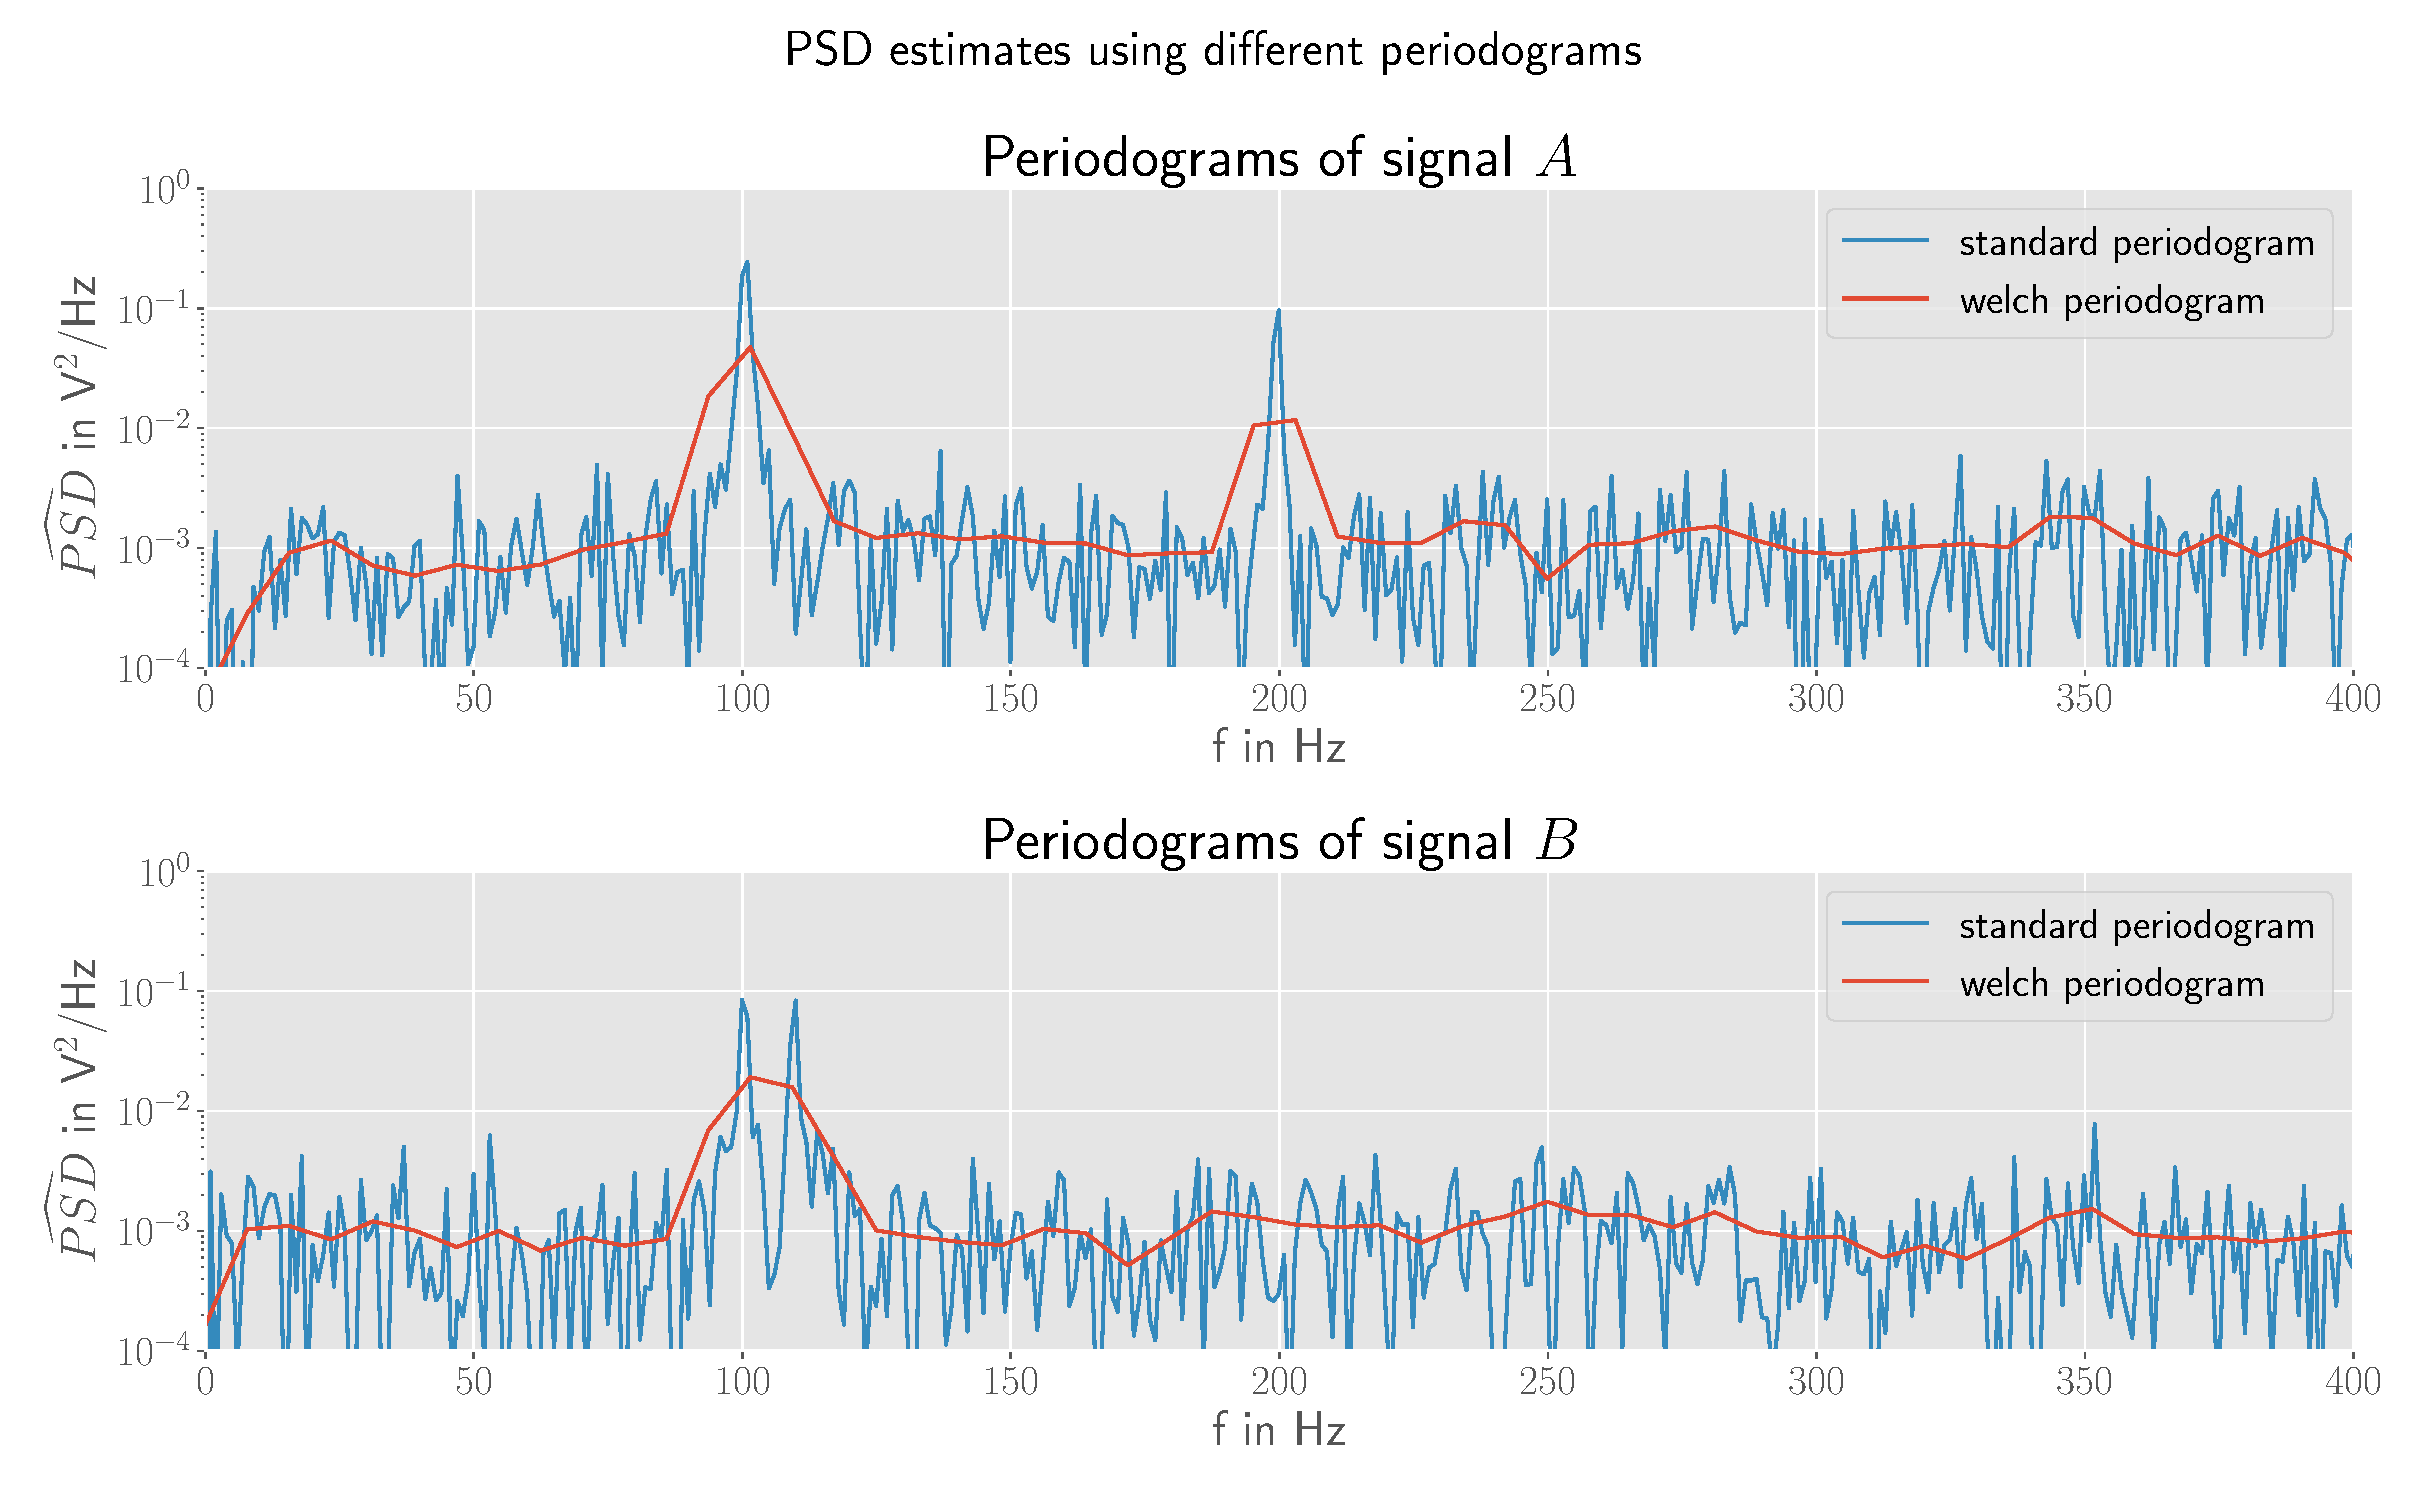
\includegraphics[width=0.764\textwidth]{graphics/welch.pdf}
\caption{Comparison of standard and welch periodograms. \inlinecodee{scipy}'s default parameters have been used for the Welch periodograms.}\label{fig:welch_exp}
\end{figure}


\begin{figure}[H]
\centering
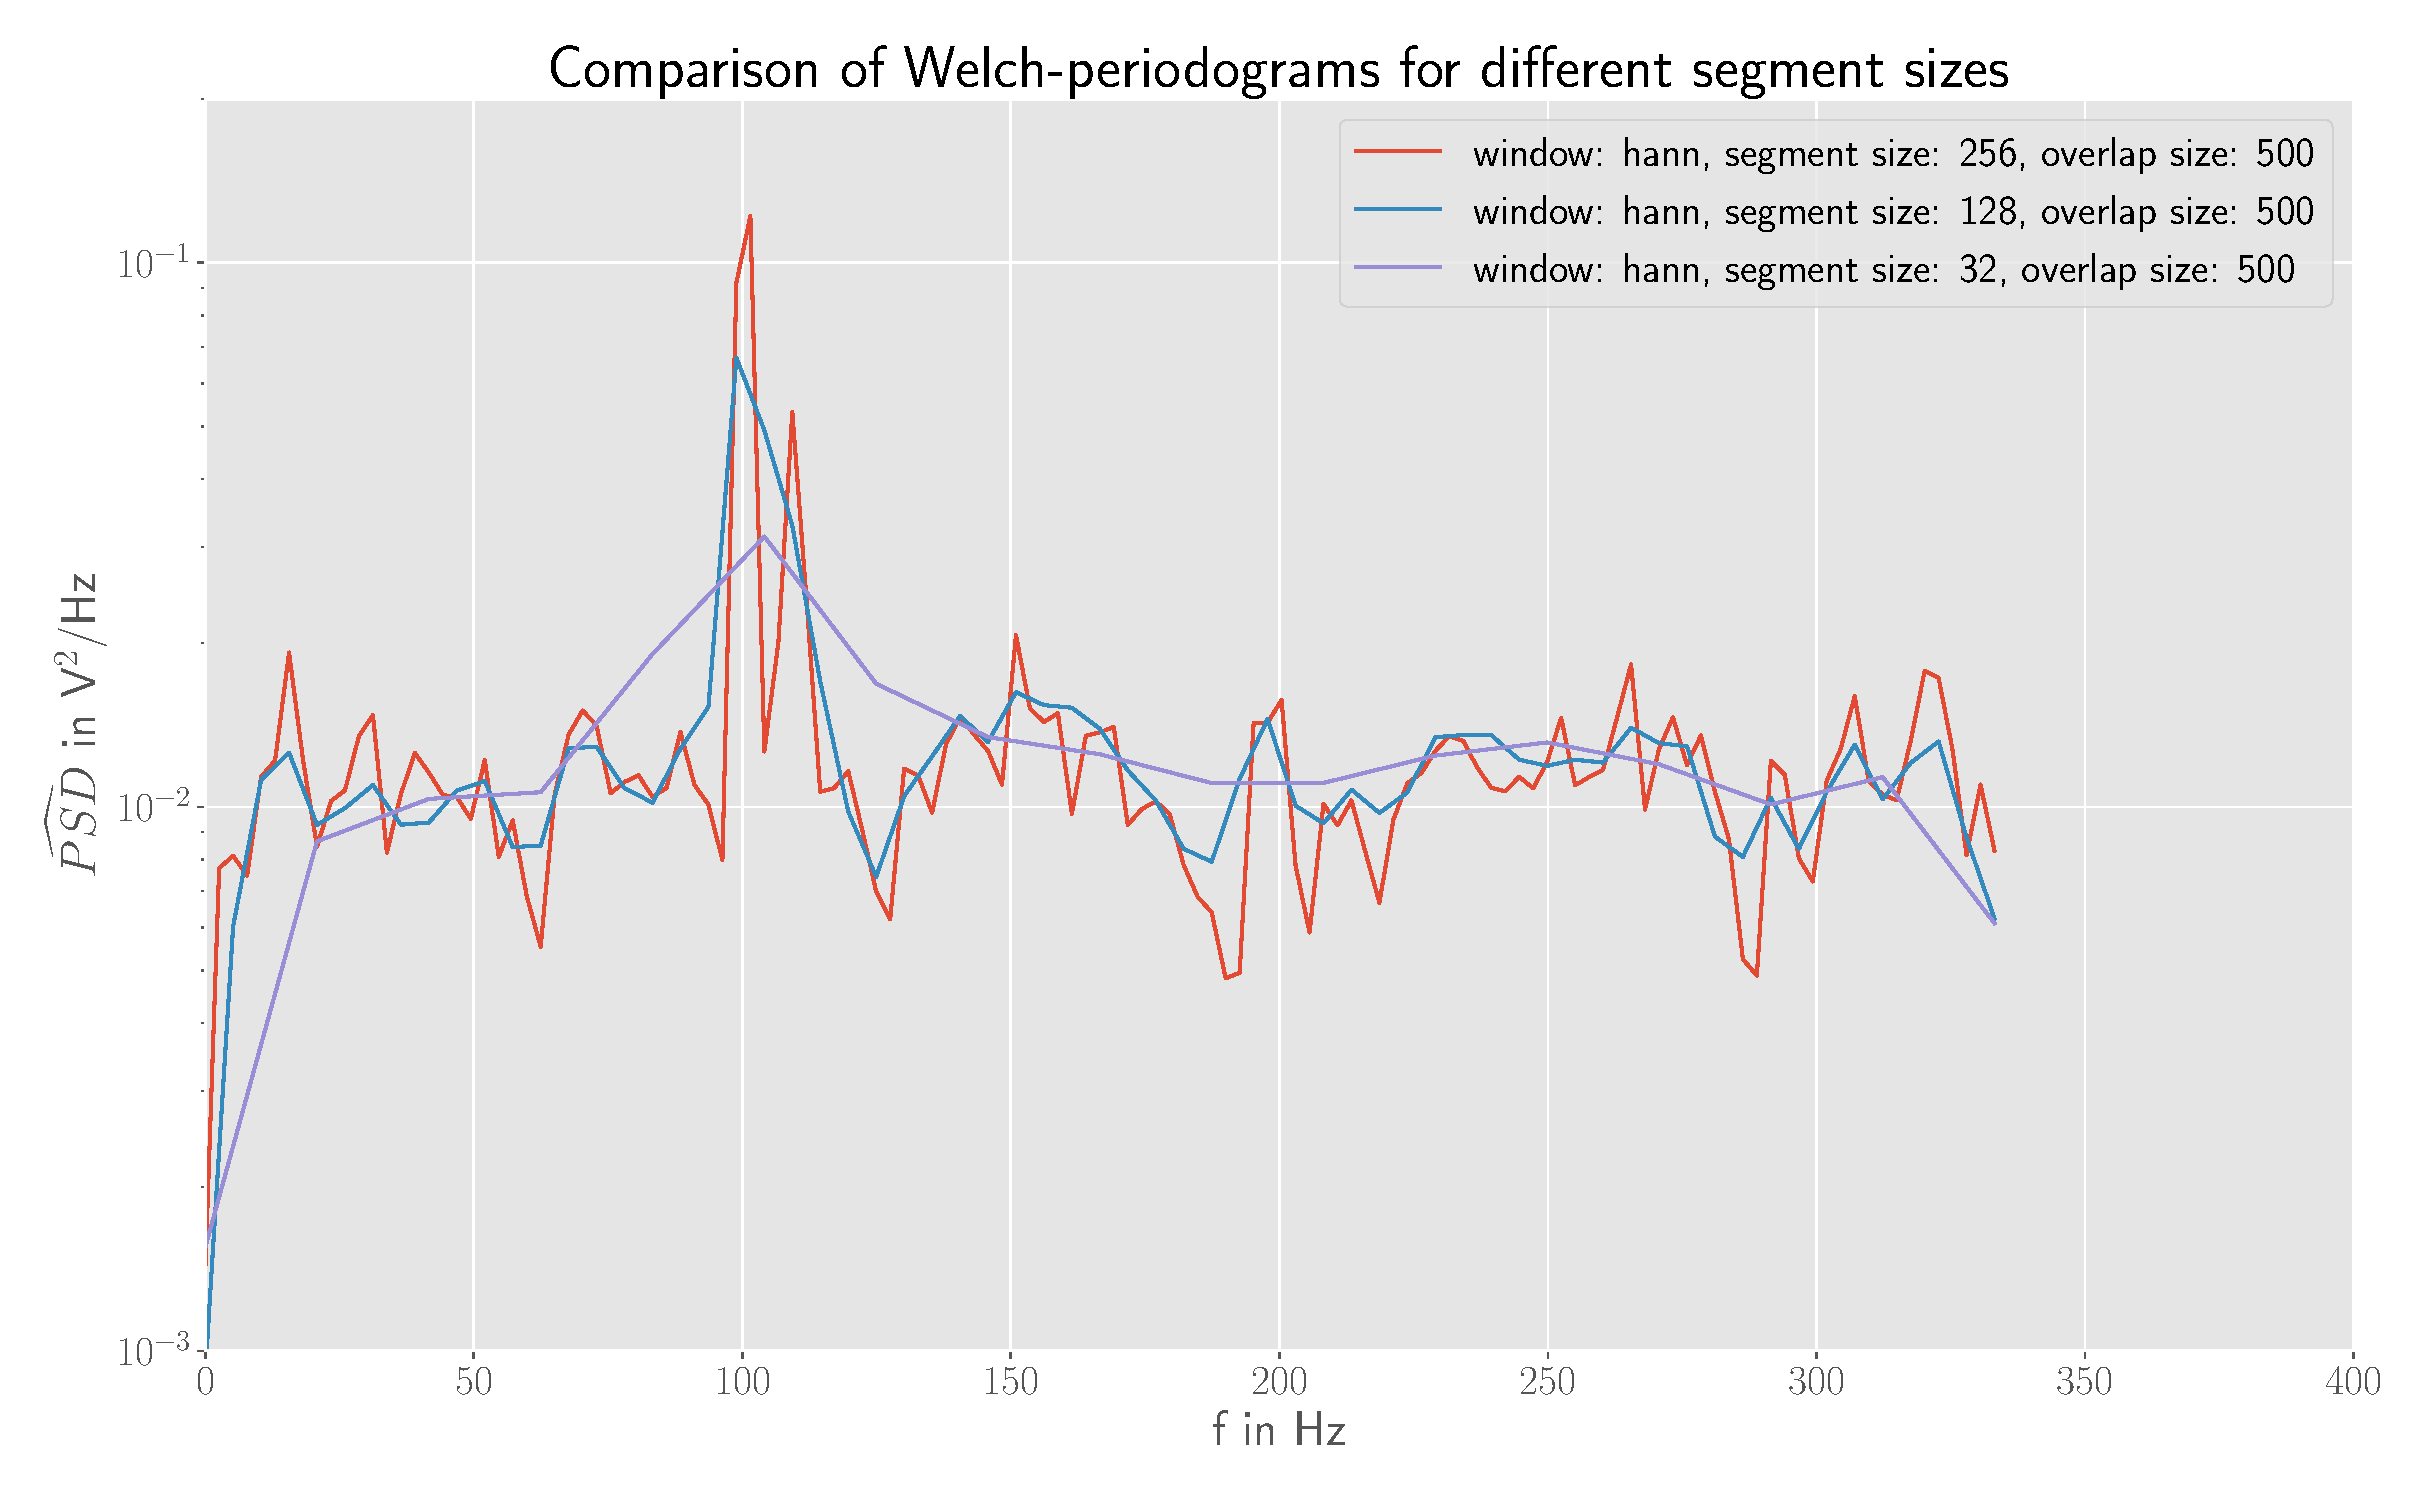
\includegraphics[width=0.764\textwidth]{graphics/welch_comp.pdf}
\caption{Comparison of different Welch segment sizes when applied to signal $B$. For code see appendix \ref{app:welch_comp}.}\label{fig:welch_comp}
\end{figure}
